\subsection{Validation using 2012 ANES}
% Here, we will look at political sophistication and competence

\begin{frame}\centering\vfill
    \begin{center}
        \begin{tikzpicture}
            \node[anchor=south west,inner sep=0] (image) at (0,0) {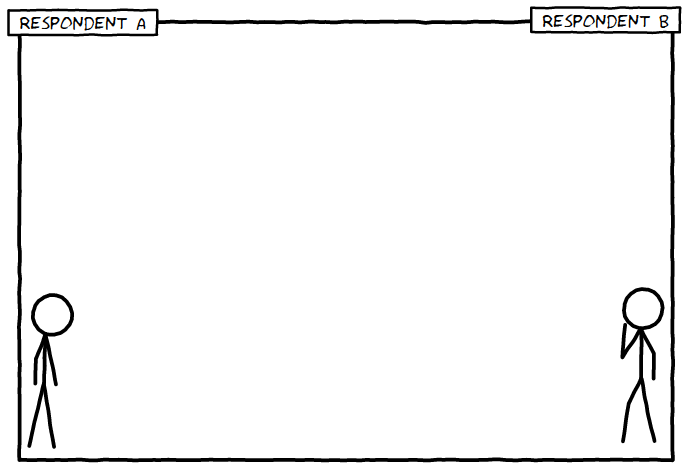
\includegraphics[width=\textwidth]{fig/Respondents_empty.png}};
            \node<2->[anchor=south west,inner sep=0] (vote) at (1.5,5) {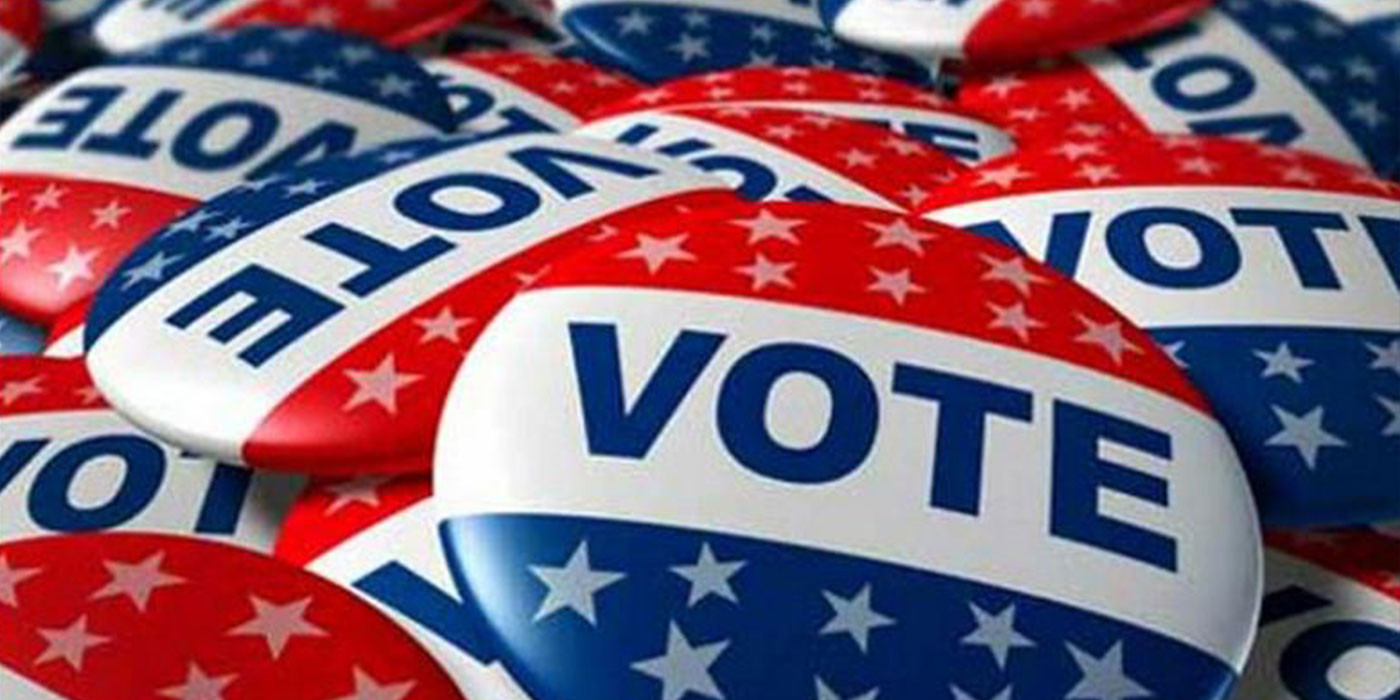
\includegraphics[width=.4\textwidth]{fig/Voting.jpg}};
            \node<3->[anchor=south west,inner sep=0] (protest) at (4.6,1.5) {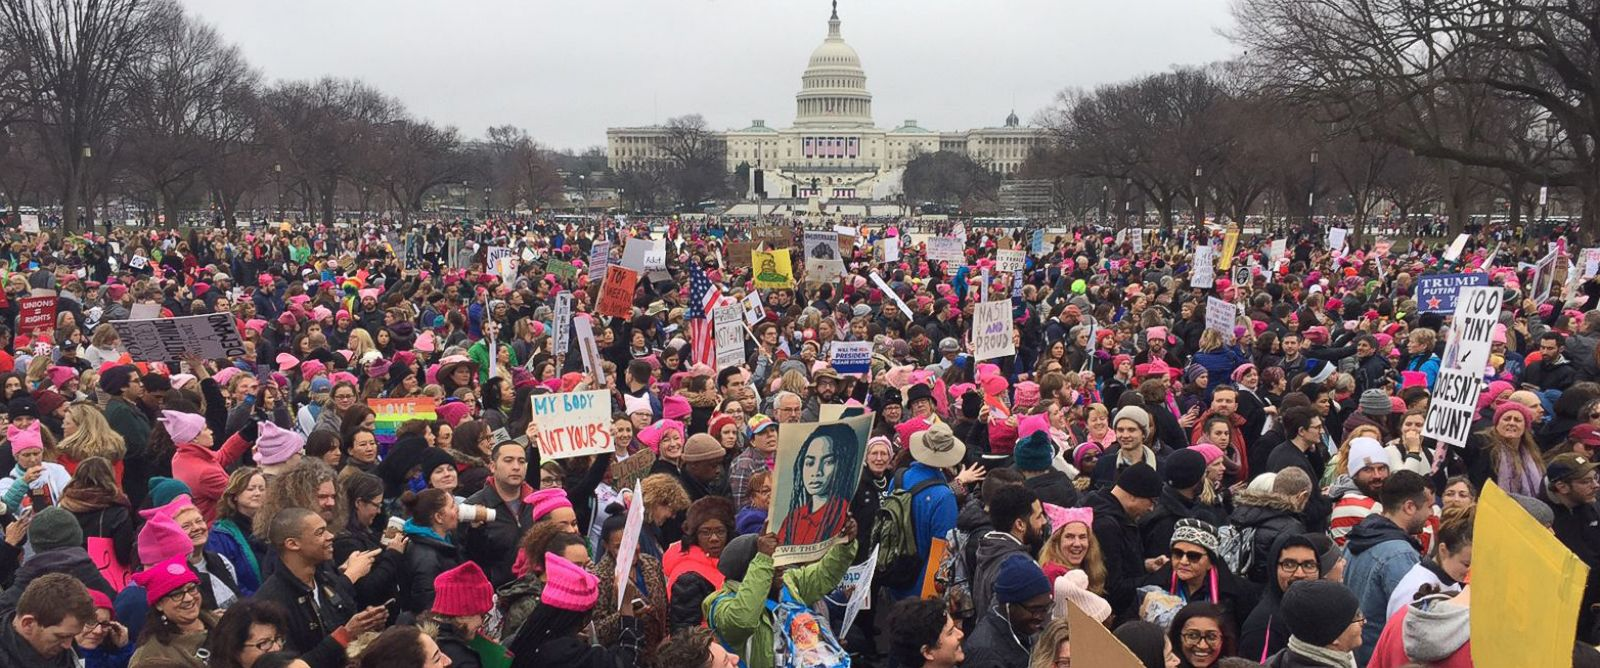
\includegraphics[width=.5\textwidth]{fig/GTY-womens-march.jpg}};
            \node<4->[anchor=south west,inner sep=0] (thinking) at (1.5,1.5) {
\includegraphics[width=.25\textwidth]{fig/gear-head-blue.png}};
            \node<5->[anchor=south west,inner sep=0] (influence) at (6.5,4.5) {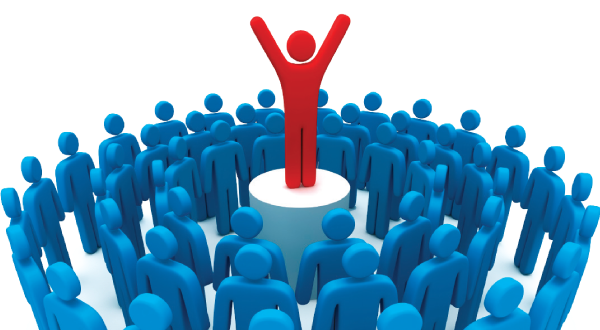
\includegraphics[width=.3\textwidth]{fig/Influence.png}};
            \node<6->[align=center,draw opacity=0,fill opacity=0.8,text opacity=1, white, fill=beamer@sbred] at (image.center) {\large Validation\\\Large 2012 American National Election Study\\\vspace{1em}\\N = 5914 (2054 f2f + 3860 online)};
        \end{tikzpicture}
    \end{center}
\end{frame}
%\item Non-response: 417, Spanish: 228

\begin{frame}{\hyperlink{engagement_joint}{Engagement and Participation}}\label{engagement}
  \begin{figure}
  \only<1>{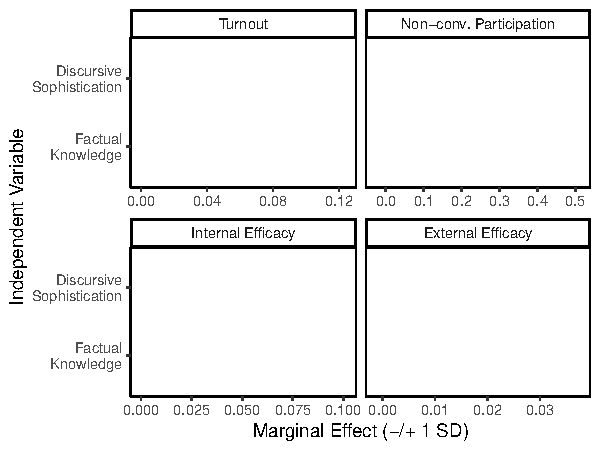
\includegraphics{../fig/knoweff_pres0.pdf}}
  \only<2>{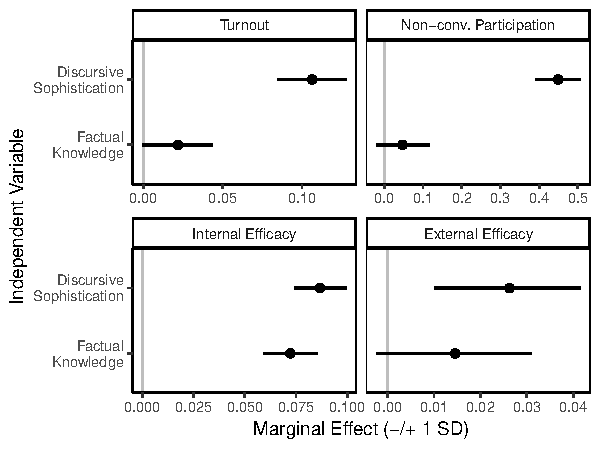
\includegraphics{../fig/knoweff_pres1.pdf}}
  \end{figure}
\end{frame}
% DISCUSS:
% Discursive sophistication is associated with:
% - \hyperlink{hetreg}{more precise candidate and party \emph{placements} on multiple \emph{policy} issues.
% -\hyperlink{prepost}{higher likelihood that citizens \emph{voted} according to their \emph{initial intention} at the time of the \emph{pre-election} interview.





